\chapter{Resultados Obtidos}
\label{Cap:Resultados}
\newcommand{\EscalaAlgumaCoisa}{0.6}

% Capítulo 4: Resultados

\section{Resultados}
\indent
\par Os resultados do projeto podem ser divididos em três grupos principais, resultados percebidos pelos usuários dos ônibus, pelos gestores das linhas e por último, por desenvolvedores que tem interesse em usar a estrutura desenvolvida.
\indent
\par O principal benefício para quem usa o sistema de ônibus de São Paulo, que pode ser sentido durante a apresentação na Eureka, foi na experiência com o mapa em tempo real e o acompanhamento das linhas do metrô dentro do dashboard. Para quem usa diariamente o serviço de transporte público da capital, poder acompanhar a situação de cada trecho dos corredores do ônibus, suas posições e no mesmo lugar, consultar como estava as linhas de metrô é algo de grande valor. Apesar da ferramenta não permitir, grande parte das pessoas expressou a vontade de consultar o dashboard em sua rotina, para conferir a situação de uma linha que é utilizada no seu trajeto, e alguns indo além, procurando explorar outros serviços, por exemplo aplicativos de carros, como Uber e Cabify.
\indent
\par Para gestores dos serviços, a possibilidade de ter em uma única ferramenta informações essenciais para a tomada de decisão durante a operação das linhas é algo fundamental, principalmente em tempo real, podendo verificar uma redução da velocidade média de algum trecho e comparar com o histórico de outros dias, e ao mesmo tempo verificar se há alguma ocorrência de um grande evento na região, ou se a situação meteorológica está afetando o tráfego na via, como em uma enchente por decorrência de fortes chuvas.
\indent
\par Também para empresa que tiver interesse de implementar a ferramenta, a arquitetura que escolhemos, de Django mais Plotly em conjunto da nossa API para a consulta dos dados armazenados, permite que com poucas linhas de Python e SQL sejam desenvolvidas novas visões que o gestor sinta a necessidade de acompanhar, coisas como volume de veículos em zonas específicas da cidade ou velocidade média em função da temperatura de uma região, por exemplo, podem ser implementadas com conhecimento básico de Python e PostgreSQL.
\indent
\par Já para os desenvolvedores que tem interesse no assunto de transporte público, a ferramenta fornece endpoints públicos, que permitem consultas que nem sempre são possíveis nos serviços oficiais, principalmente no caso das APIs da SPTrans. Foram desenvolvidos caminhos que permitem não só consultas em tempo real, mas também informações históricas, que inclusive durante o desenvolvimento do projeto fizeram falta para análises mais profundas. As informações são disponibilizadas de forma agnóstica por meio de APIs, com as consultas podendo ser feitas com o uso de qualquer linguagem que suporte requisições HTTP, não sendo limitada pelo uso do Python ou SQL. Além disso, todos os dados já são tratados antes de serem armazenados, mesmo em situações como dos Eventos, em que a captura deles foi feita através de raspagem de tela, com auxílio do Selenium.

\begin{figure}[H]
    \centering
    \caption{Tela do dashboard}
    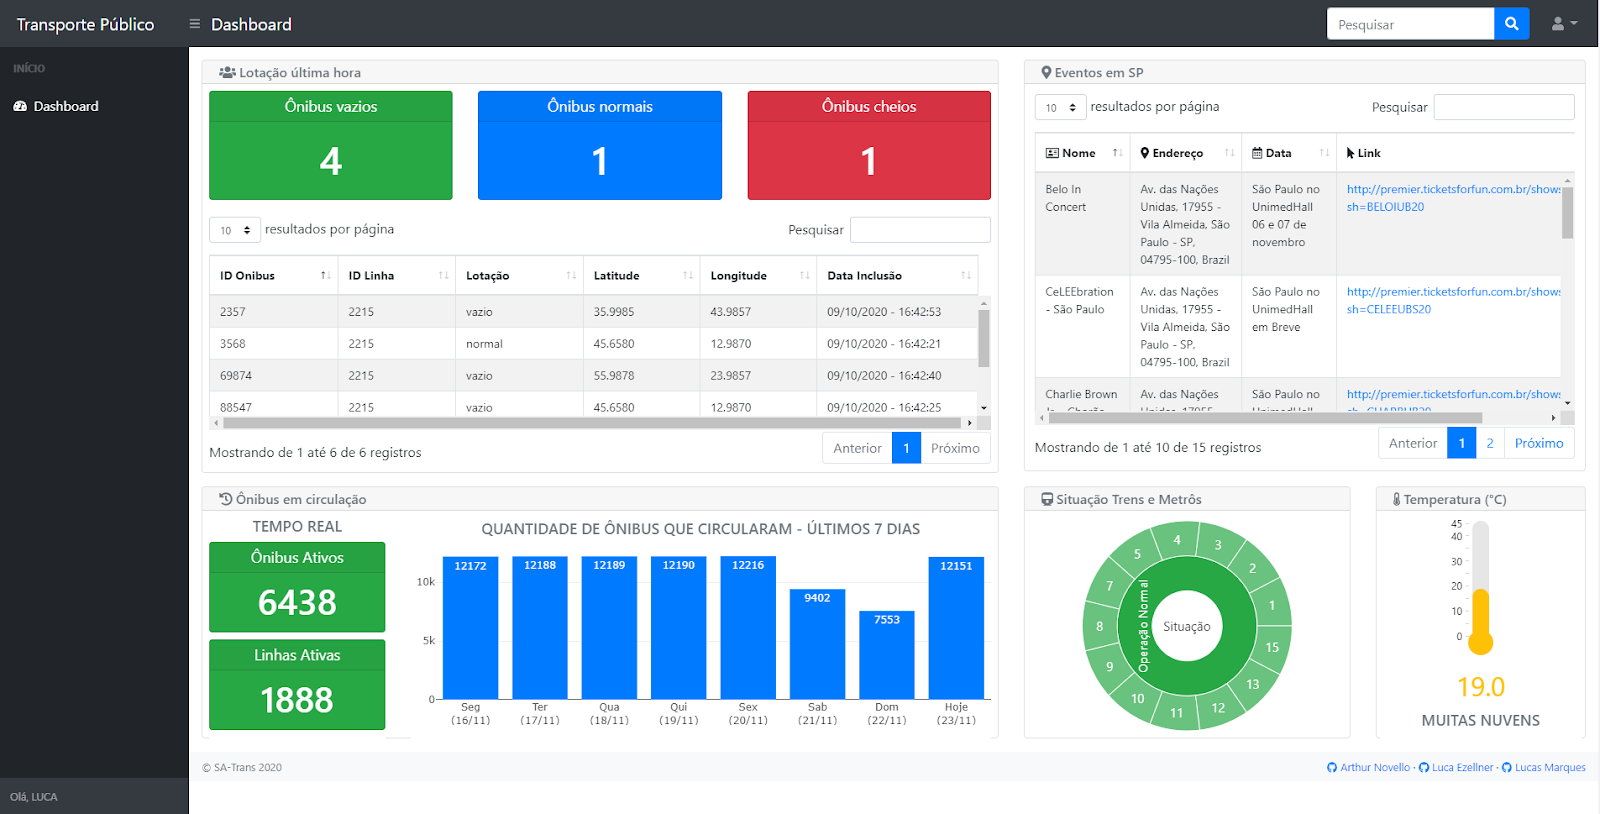
\includegraphics[width=1.0\linewidth]{Imagens/dashboard1.png}
    \caption*{Fonte: Arquivo dos autores (2020)}
    \label{telaDashboard1}
\end{figure}

\begin{figure}[H]
    \centering
    \caption{Tela do dashboard}
    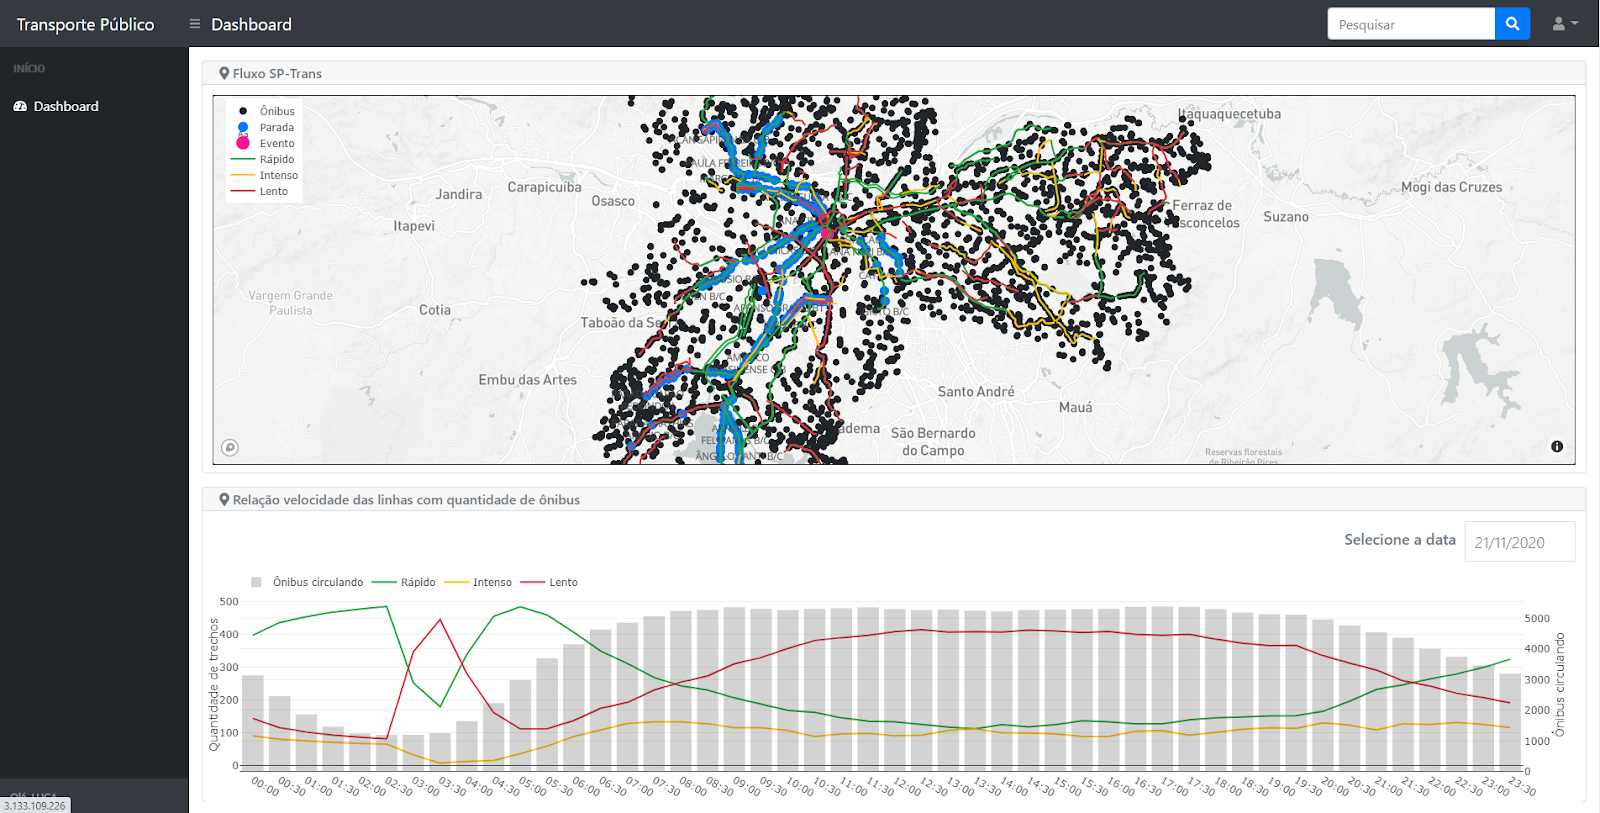
\includegraphics[width=1.0\linewidth]{Imagens/dashboard2.png}
    \caption*{Fonte: Arquivo dos autores (2020)}
    \label{telaDashboard2}
\end{figure}









